\documentclass[letterpaper,10pt,onecolumn]{article}
\usepackage[spanish]{babel}
\usepackage[utf8x]{inputenc}
\usepackage{amsfonts}
\usepackage{amsthm}
\usepackage{amsmath}
\usepackage{mathrsfs}
\usepackage{empheq}
\usepackage{enumitem}
\usepackage[pdftex]{color,graphicx}
\usepackage{hyperref}
\usepackage{listings}
\usepackage{calligra}
\usepackage{algpseudocode} 
\DeclareMathAlphabet{\mathcalligra}{T1}{calligra}{m}{n}
\DeclareFontShape{T1}{calligra}{m}{n}{<->s*[2.2]callig15}{}
\newcommand{\scripty}[1]{\ensuremath{\mathcalligra{#1}}}
\lstloadlanguages{[5.2]Mathematica}
\setlength{\oddsidemargin}{0cm}
\setlength{\textwidth}{490pt}
\setlength{\topmargin}{-40pt}
\addtolength{\hoffset}{-0.3cm}
\addtolength{\textheight}{4cm}

\begin{document}
\begin{center}



\includegraphics[width=490pt]{header.png}\\[0.5cm]

\textsc{\LARGE Taller 8 - F\'isica I (FISI-1018) - 2016-10}\\[0.5cm]

\textsc{\Large{Profesor: Jaime Forero}} \\[0.5cm]

\noindent\textsc{Ejercicios correspondiente a la clase complementaria de la semana del 14 de Marzo del 2016.}\\[0.5cm]
\end{center}

\noindent\textsc{Nota:} 
Los primeros tres ejercicios deben ser
entregados {\bf al comienzo} de la clase complementaria. Los \'ultimos
cuatro deben ser trabajados {\bf durante} la complementaria. 

La numeraci\'on
hace referencia al texto gu\'ia: \textit{F\'isica Universitaria Volumen
  1 (Sears-Semansky)}, decimotercera edici\'on, Pearson.

\begin{enumerate}

% aqui vienen los tres ejercicios "faciles"
\item Ejercicio 6.44. Resorte partido a la mitad %Juan Carlos
\item Ejercicio 7.38 Canica que se mueve sobre el eje x. % Jaime
\item Se cuelga un resorte del techo de un ascensor en reposo. Su longitud libre es de $30cm$ y su constante elástica de $500N/m$. Se coloca un cuerpo en el extremo libre del resorte y éste se estira $10cm$, quedando en reposo. Un pasajero observa que, durante algunos segundos el estiramiento del resorte corresponde a $13cm$. 
\begin{enumerate}
\item
Realice el diagrama de cuerpo libre del sistema. Considere los casos cuando el asensor esta en reposo  y cuando esta acelerado. 
 \item
¿cuál es la aceleración del ascensor (tenga en cuenta el estiramiento del resorte)?
\end{enumerate}
%Miguel
% aqui vienen los cuatro ejercicios "dificiles"
\item Ejercicio 7.42 Sistema bloque-resorte y un plano inclinado %Juan Carlos
\item Problema 7.63 Esquiadora que pierde contacto.. %Jaime
\item Problema 7.56 Cohete sobre una rampa. % Jaime
\item Un carro de montaña rusa se lanza desde una altura $h$, que velocidad tienen el carro en el punto $A$ (Según la figura). ¿Cuál es la altura mínima de la cual se debe lanzar el carro para que llegue hasta el punto $A$? (La respuesta debe estar dada en términos de R). 
\begin{figure}[h]
\begin{center} 
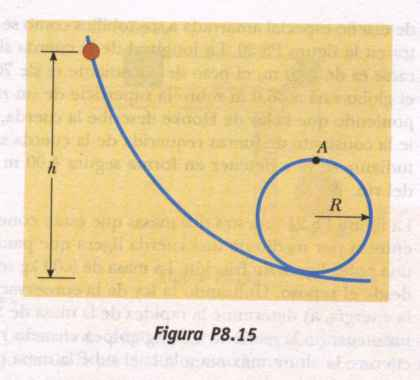
\includegraphics[scale=1.5]{montanarusa.jpg} 
\end{center} 
\end{figure}
%Miguel
 \end{enumerate}
 

\end{document}


\begin{figure}[h]
\begin{center} 
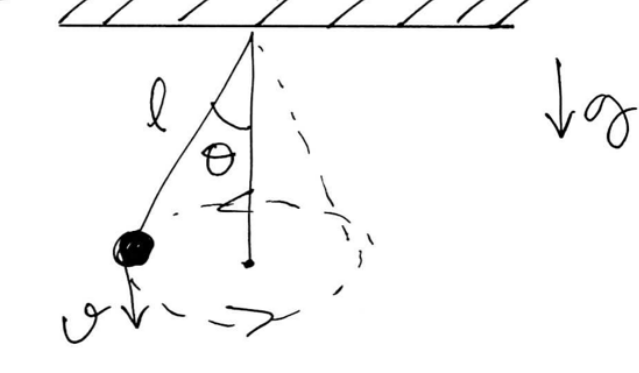
\includegraphics[scale=0.25]{conico.png} 
\caption{\label{fig:conico}Figure para el problema \ref{conico}}
\end{center} 
\end{figure}

\begin{figure}[!h]
\begin{center}
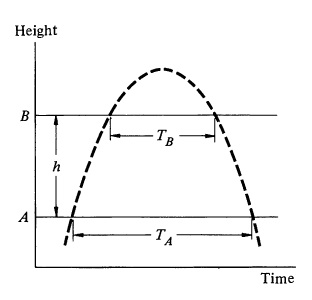
\includegraphics[scale=0.7]{altura.jpg} 
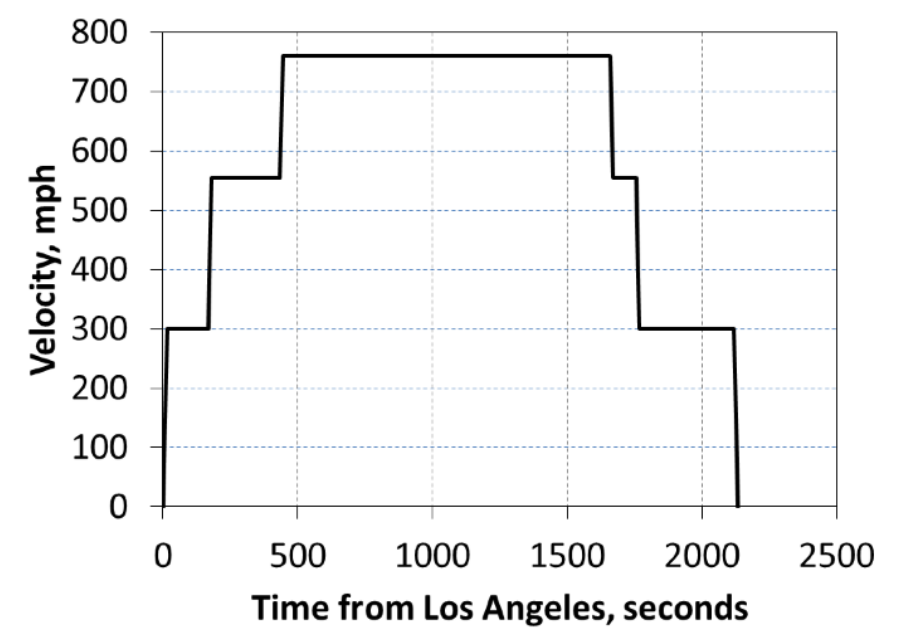
\includegraphics[scale=0.3]{hyperloop.png} 
\end{center}
\caption{Izquierda: diagrama para el ejercicio recomendado 3. Derecha: diagrama para el ejercicio recomendado 4.}
\label{fig:tiro}
\end{figure}





